% Options here are passed to the article class.
% Most common options: 10pt, 11pt, 12pt
\documentclass[10pt]{datasheet}

% Input encoding and typographical rules for English language
\usepackage[utf8]{inputenc}
\usepackage[english]{babel}
\usepackage[english]{isodate}

% tikz is used to draw images in this example, but you can
% also use \includegraphics{}.
\usepackage{graphicx}

% These define global texts that are used in headers and titles.
\title{IM03: Compact Disk Drive Temp Storage}
\author{Obi, Crain, PallaPalla, xXOpticNerveXx, JayRoi}
\tags{item-memory, disk-drive, temp-storage}
\date{21 December 2023}
\revision{Revision 1}
\begin{document}
\maketitle

\section{Features}

\begin{itemize}
\item{Stores 32 boxes in each double chest for high density}
\item{8 bit address, up to 256 boxes}
\item{Built in isBox check for easy pair detection}
\item{Safety feature checks if chest is reset properly}
\item{Safety feature checks if placeholder items are missing}
\end{itemize}

\section{Applications}

\begin{itemize}
\item{Dynamic sorting partial box merging loop}
\end{itemize}

\section{General Description}

The IM03 Compact Disk Drive Temp Storage is a device that stores boxes in a temporary storage system. The device is designed to be used in a dynamic sorting system to merge partial boxes. To use, set an 8 bit address and input a box. The drive will iterate through the boxes in the right chest to find a box already stored in the system. If a box is found, both boxes are outputted. If no box is found, the input box is stored in the drive for later pairing. The drive can store up to 256 boxes (one per address) in 8 double chests. \href{https://www.youtube.com/watch?v=_OpecWSo2yc}{Youtube video}

\vfill\break

\begin{figure}[h]
    \centering
    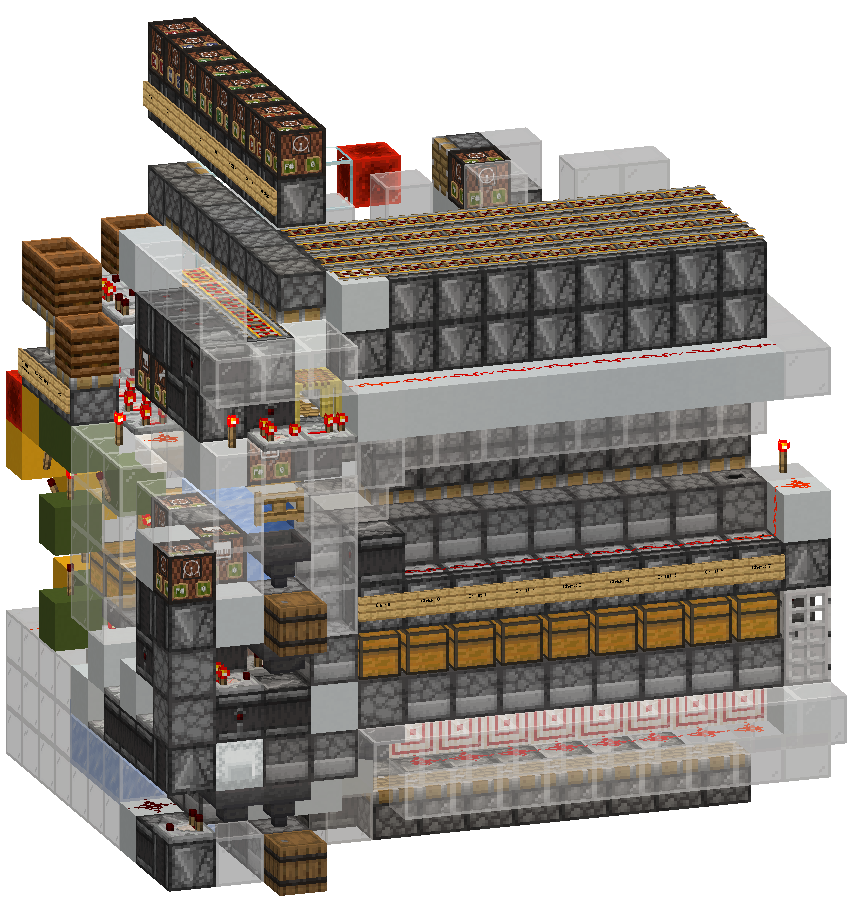
\includegraphics[width=0.48\textwidth]{diskdrive.png}
    \caption{\centering Compact Disk Drive Temp Storage}
\end{figure}

% For wide tables, a single column layout is better. It can be switched
% page-by-page.
\onecolumn

\section{Device Specifications}

\begin{table}[h]
    \caption{Inputs}
    \begin{tabularx}{\textwidth}{l | c | X}
        \thickhline
        \textbf{Name} & \textbf{Range} & \textbf{Description} \\
        \hline
        Address Bits 0-7 & 0-1 & Binary address of box \\
        \hline
        Box input & box & Box input. Usually a partial box from a splitter. \\
        \hline
        Manual shutoff & 0-1 & Manually shuts off device. \\
        \thickhline
\end{tabularx}
\end{table}

\begin{table}[h]
    \caption{Outputs}
    \begin{tabularx}{\textwidth}{l | c | X}
        \thickhline
        \textbf{Name} & \textbf{Range} & \textbf{Description} \\
        \hline
        Box outputs 1-2 & box & Box output. Only outputs boxes with the other output simultaneously when a match is found. \\
        \hline
        isResetProper & 0-1 & Indicates disk drive is reset properly for next use. \\
        \hline
        hasCodeItems & 0-1 & Indicates disk drive has enough placeholder items for next use. \\
        \hline
        hasBox & 0-1 & Indicates disk drive has input box \\
        \hline
        \thickhline
\end{tabularx}
\end{table}

\begin{table}[h]
    \caption{Device Specifications}
    \begin{tabularx}{\textwidth}{l | c c c | c | X}
        \thickhline
        \textbf{Parameter} & \textbf{Min.} & \textbf{Typ.} & \textbf{Max.} &
        \textbf{Unit} & \textbf{Conditions} \\
        \hline
        Throughput  & 281 & - & 790 & gt & Normal Usage \\
        \hline
        Minimum Latency & 143 & - & 391 & gt & From input to pair output \\
        \hline
        MC Version & 1.16 & 1.17.1 & - & MCV & Latest version at time of writing: 1.20.4\\
        \hline
        Dimensions & & 14 x 13 x 10 & & Blocks & \\
        \thickhline
\end{tabularx}
\end{table}
\newpage
\section{Testing Data}
\begin{table}[h]
\caption{Executed Tests}
\begin{tabularx}{\textwidth}{l | X}
    \thickhline
    \textbf{Test} & \textbf{Result} \\
    \hline
    Pair generation test & Device was able to produce pairs corresponding to the address. \\
    \thickhline
\end{tabularx}
\end{table}

\section{Download Information}
\begin{table}[h]
    \caption{Download Information}
    \begin{tabularx}{\textwidth}{l | l | l | X}
        \thickhline
        \textbf{Identifier} & \textbf{MC} & \textbf{File} & \textbf{Description} \\
        \hline
        IM03 & 1.17.1 & \href{https://github.com/Soontech-Annals/Archive/blob/8413f90a054b6c415703bae02badeba7541344f6/Archive/item-memory/IM03\%20Compact\%20Disk\%20Drive\%20Temp\%20Storage/IM03\_Compact\_Disk\_Drive\_Temp\_Storage.zip?raw=1}{IM03\_Compact\_Disk\_Drive\_Temp\_Storage.zip} & World download of device. \\
        \hline
        IM03 & 1.17.1 & \href{https://github.com/Soontech-Annals/Archive/blob/8413f90a054b6c415703bae02badeba7541344f6/Archive/item-memory/IM03\%20Compact\%20Disk\%20Drive\%20Temp\%20Storage/IM03\_Compact\_Disk\_Drive\_Temp\_Storage.litematic?raw=1}{IM03\_Compact\_Disk\_Drive\_Temp\_Storage.litematic} & Schematic of device. Inventories included. \\
        \hline
        \thickhline
    \end{tabularx}
\end{table}

\end{document}

